\documentclass{article}\usepackage[]{graphicx}\usepackage[]{color}
% maxwidth is the original width if it is less than linewidth
% otherwise use linewidth (to make sure the graphics do not exceed the margin)
\makeatletter
\def\maxwidth{ %
  \ifdim\Gin@nat@width>\linewidth
    \linewidth
  \else
    \Gin@nat@width
  \fi
}
\makeatother

\definecolor{fgcolor}{rgb}{0.345, 0.345, 0.345}
\newcommand{\hlnum}[1]{\textcolor[rgb]{0.686,0.059,0.569}{#1}}%
\newcommand{\hlstr}[1]{\textcolor[rgb]{0.192,0.494,0.8}{#1}}%
\newcommand{\hlcom}[1]{\textcolor[rgb]{0.678,0.584,0.686}{\textit{#1}}}%
\newcommand{\hlopt}[1]{\textcolor[rgb]{0,0,0}{#1}}%
\newcommand{\hlstd}[1]{\textcolor[rgb]{0.345,0.345,0.345}{#1}}%
\newcommand{\hlkwa}[1]{\textcolor[rgb]{0.161,0.373,0.58}{\textbf{#1}}}%
\newcommand{\hlkwb}[1]{\textcolor[rgb]{0.69,0.353,0.396}{#1}}%
\newcommand{\hlkwc}[1]{\textcolor[rgb]{0.333,0.667,0.333}{#1}}%
\newcommand{\hlkwd}[1]{\textcolor[rgb]{0.737,0.353,0.396}{\textbf{#1}}}%
\let\hlipl\hlkwb

\usepackage{framed}
\makeatletter
\newenvironment{kframe}{%
 \def\at@end@of@kframe{}%
 \ifinner\ifhmode%
  \def\at@end@of@kframe{\end{minipage}}%
  \begin{minipage}{\columnwidth}%
 \fi\fi%
 \def\FrameCommand##1{\hskip\@totalleftmargin \hskip-\fboxsep
 \colorbox{shadecolor}{##1}\hskip-\fboxsep
     % There is no \\@totalrightmargin, so:
     \hskip-\linewidth \hskip-\@totalleftmargin \hskip\columnwidth}%
 \MakeFramed {\advance\hsize-\width
   \@totalleftmargin\z@ \linewidth\hsize
   \@setminipage}}%
 {\par\unskip\endMakeFramed%
 \at@end@of@kframe}
\makeatother

\definecolor{shadecolor}{rgb}{.97, .97, .97}
\definecolor{messagecolor}{rgb}{0, 0, 0}
\definecolor{warningcolor}{rgb}{1, 0, 1}
\definecolor{errorcolor}{rgb}{1, 0, 0}
\newenvironment{knitrout}{}{} % an empty environment to be redefined in TeX

\usepackage{alltt}
\usepackage{Sweave}
\usepackage{float}
\usepackage{graphicx}
\usepackage{tabularx}
\usepackage{siunitx}
\usepackage{amssymb} % for math symbols
\usepackage{amsmath} % for aligning equations
\usepackage{textcomp}
\usepackage{mdframed}
\usepackage[T1]{fontenc}
\usepackage{subcaption}
\usepackage{natbib}
\bibliographystyle{..//refs/styles/besjournals.bst}
\usepackage[small]{caption}
\setlength{\captionmargin}{30pt}
\setlength{\abovecaptionskip}{0pt}
\setlength{\belowcaptionskip}{10pt}
\captionsetup{justification=raggedright,singlelinecheck=false}
\topmargin -1.5cm        
\oddsidemargin -0.04cm   
\evensidemargin -0.04cm
\textwidth 16.59cm
\textheight 21.94cm 
%\pagestyle{empty} %comment if want page numbers
\parskip 7.2pt
\renewcommand{\baselinestretch}{1.5}
\parindent 0pt
\usepackage{lineno}
\linenumbers

%cross referencing:
\usepackage{xr}
\usepackage{xr-hyper}
\externaldocument{/Users/CatherineChamberlain/Documents/git/microclimates/docs/micro_supp}

\newmdenv[
  topline=true,
  bottomline=true,
  skipabove=\topsep,
  skipbelow=\topsep
]{siderules}
\IfFileExists{upquote.sty}{\usepackage{upquote}}{}
\begin{document}

\noindent\textbf{\Large{Comparing spring phenology in an urban arboretum versus rural forested site and implications for forecasting}}

\noindent Authors:\\
C. J. Chamberlain $^{1,2}$ \& E. M. Wolkovich $^{1,2,3}$
\vspace{2ex}\\
\emph{Author affiliations:}\\
$^{1}$Arnold Arboretum of Harvard University, 1300 Centre Street, Boston, Massachusetts, USA; \\
$^{2}$Organismic \& Evolutionary Biology, Harvard University, 26 Oxford Street, Cambridge, Massachusetts, USA; \\
$^{3}$Forest \& Conservation Sciences, Faculty of Forestry, University of British Columbia, 2424 Main Mall, Vancouver, BC V6T 1Z4\\
\vspace{2ex}
$^*$Corresponding author: 248.953.0189; cchamberlain@g.harvard.edu\\

\noindent \emph{Keywords:} phenology, climate change, forest communities, microclimate, urban heat island, growing degree days\\

\renewcommand{\thetable}{\arabic{table}}
\renewcommand{\thefigure}{\arabic{figure}}
\renewcommand{\labelitemi}{$-$}
\setkeys{Gin}{width=0.8\textwidth}

%%%%%%%%%%%%%%%%%%%%%%%%%%%%%%%%%%%%%%%%%%%%%%%
%%%%%%%%%%%%%%%%%%%%%%%%%%%%%%%%%%%%%%%%%%%%%%%


\newpage
\section*{Abstract} % (274/300)
Understanding and predicting plant phenology in temperate forests is critical for forecasting important processes such as carbon storage, especially with climate change and urbanization shifting many phases including budburst and leafout. One major forecasting method for phenology is the growing degree day (GDD) model, allows researchers to track heat accumulation. GDD models typically assume that the GDD threshold for a species or even functional type is constant, but increasing evidence suggests otherwise. Climate can vary a lot on small spatial scales and recent studies suggest that fine-scale climate may matter to phenology. Here, we use observations from one urban arboretum and one rural forested site to assess GDDs until budburst using two methods for measuring climate data (i.e., weather station data and hobo logger data). We additionally incorporate simulations to better interpret our results and conclude with a series of simulated forecasts to estimate changes in these GDD model estimates. Our results suggest the urban arboretum site requires fewer GDDs until budburst and may have stronger microclimate effects than the rural forested site though these effects diminish with the use of hobo loggers. Additionally, we find that GDD models may become less accurate with warming and GDDs begin to accumulate at a faster rate. Our findings suggest we need to either use a method that is less reliant on accumulated, climatological sums or we must scrutinize results through the use of mixed models and simulated data as we demonstrate here.

\section*{Introduction}

Understanding and predicting plant phenology in temperate deciduous forests is critical as it both shapes community structure and also influences major ecosystem services such as resource and forest management. Climate change and urbanization are advancing spring timing---such as budburst and leafout, which  are strongly cued by temperature, resulting in longer growing seasons \citep{Chuine2001} which ultimately impacts these services. Spring budburst timing can have cascading effects to pollinators \citep{Boggs2012, Pardee2017}, on albedo \citep{Williamson2016}, and on carbon dynamics \citep{Richardson2013}. Temperate forests sequester carbon and help mitigate the negative effects of climate change and---with earlier spring phenology and longer growing seasons---there has been an increase in carbon uptake \citep{Keenan2014}. Because of the importance of phenology, forecasting it accurately with climate change is a major and important aim across several fields of science \citep{Moorcroft2001,Taylor2020,Yu2016,Zhao2012}.
  
One major forecasting method across all these fields is the growing degree day model. The growing degree day (GDD) model allows researchers to track heat accumulation to measure spring budburst \citep{Cook2012,Crimmins2020,Phillimore2013,Schwartz2006,Vitasse2011}. The GDD model simply sums temperatures above a certain threshold---often around 0$^{\circ}$C for forested trees as estimates are proven to be more accurate \citep{Man2010}---and different species often require a different number of GDDs to leaf out. GDDs accumulate at a faster rate when mean temperatures are higher, thus different sites or different climate measurement methods may record different GDD thresholds for budburst. Integrating the GDD model successfully is essential for predicting the effects of climate change on systems where the climate is rapidly changing, including temperate forests. 
  
We often assume in GDD models that the GDD required for a species, or even a suite of species (e.g., plant functional types) is constant, but increasing evidence suggests it may not be. The plasticity of phenology means that the same individual exposed to different climates will leafout at a very different time. Decades of work show that chilling---related to winter temperatures---and photoperiod can shift the GDD a plant needs for the same event \citep{Basler2012,Chuine2010,Zohner2016}. Spring phenology also has a genetic component, and the required chilling, photoperiod and GDD can vary by population \citep{Scotti2004,Cuervo-Alarcon2018}. Though this genetic effect seems smaller than for other phenological events \citep{McKown2013,Satake2013}.

Climate, both on a larger or smaller scale, helps determine the role of chilling and photoperiod. On a large scale, there are climate gradients across space (i.e., latitudinal or continentality effects), but also gradients due to anthropogenic impact. Urbanization has led to the formation of urban heat islands, which have been shown to affect plant phenology and lead to earlier spring leafout \citep{Meng2020}. Because urban sites strongly contribute to carbon sequestration \citep{Ziter2018}, these trends are crucial to understand in order to predict plant development with warming. 
  
Increasingly, researchers have suggested that urban environments provide a natural laboratory for assessing the effects of warming on temperate tree and shrub species as these sites are warming at a faster rate than more rural habitats \citep{Pickett2011, Grimm2008}. Additionally urban sites often house arboreta or botanical gardens that often contribute long-term records \citep{Zohner2014} or are used for experiments on phenology \citep{Ettinger2018}. Arboreta and botanical gardens offer a unique lens to investigate climate change and local adaptation studies by incorporating varying seed sources---or provenance locations---thus they mimic common garden experiments \citep{Primack2009}. It is essential that we have a better understanding if results from such urban sites directly translate to more natural forests. 
  
Climate on a smaller scale may also be important to consider. Climate can vary significantly on small spatial scales \citep[][e.g., as much as 2.6$^{\circ}$C between sensors at the same vineyard or up to 6.6$^{\circ}$C within 1 km spatial units in northern Europe]{deResseguier2020,Lenoir2013}. Thus, increasing evidence suggests that fine-scale climate may matter to phenology \citep{Lembrechts2019}. Additionally, temperature variation at the bud level is shown to affect budburst timing within an individual canopy \citep{Lembrechts2019}. To facilitate scaling and minimize error due to these fine-scal climatic effects (i.e., microclimate effects), researchers often deploy standalone weather loggers---such as HOBO sensors---which may provide higher resolution weather data \citep{Schwartz2013a,Whiteman2000}. Though deploying temperature loggers is not always feasible, especially when investigating large spatiotemporal shifts in GDDs. 
  
Provenance location may also matter, though evidence is lacking for spring phenological phases \citep{Aitken2015, McKown2013}. There is large debate over the role of provenance latitude on budburst initiation and the associated shifts in phenological cue use. Some studies suggest that: (1) species from lower latitudes will be more reliant on photoperiod with climate change \citep{Zohner2016}, (2) photoperiod will slow or constrain range expansion \citep{Saikkonen2012}, (3) all species will rely on photoperiod more as winters warm \citep{Way2015}, and (4) lower latitude species will require both strong photoperiod cues and more forcing in order to compensate for the lack of chilling but photosensitivity may be more important at the cold trailing edge for range expansion to occur \citep{Gauzere2017}. Many arboreta keep diligent acquisition records, providing visitors and scientists information on seed sources \citep{Dosmann2006}, and the potential to test such provenance effects.

Here, we aimed to address the following hypotheses: (1) required GDD in an urban arboreta will vary from a rural forested site. We predicted lower chilling in the urban site could lead to greater required GDD, (2) individuals with provenance latitudes from more northern locations require fewer GDDs to budburst, and (3) microclimates will lead to variation in GDD within sites,. We tested these in one urban arboretum and one rural forested site and we additionally incorporated simulations to help better interpret our results. 

\section*{Methods}
\subsection*{Sites}
We chose two sites---one urban arboretum and one forest---with overlapping species and climates to compare the number of growing degree days to budburst across species. The urban site is in Boston, MA at the Arnold Arboretum of Harvard University (42$^{\circ}$17' N -71$^{\circ}$8' W). The Arnold Arboretum is 281 acres, contains 3825 woody plant taxa from North America, Europe and Asia and has an elevation gain of approximately 96m. The forest site is in Petersham, MA at the Harvard Forest (42$^{\circ}$31'53.5' N -72$^{\circ}$11'24.1' W). The Harvard Forest is 1446 acres and has a range of elevation of 220-410m. 

\subsection*{Simulations}
We simulated test data in order to assess our model output results, especially our inference on teasing out effects of microclimates versus provenance versus potential differences across weather station and hobo logger data. Our simulations were designed to test the following potential effects: (1) urban environments require more GDDs, (2) presence of provenance effects (i.e., there were multiple provenance latitudes at the urban arboretum site but only one at the rural forest site), (3) presence of microclimates (at one or both sites) accurately measured by hobo loggers and (4) weather stations or hobo loggers are effectively `noisier' data for GDD models compared to the other. 

To run our simulations, we assumed each species needed a different GDD (drawing each species' requirement from a normal distribution). We then modeled climate data by again establishing a random distribution around a mean temperature for each site. Using this climate data, we found the day of budburst when the unique GDD threshold was met for each individual. To test that urban sites require more GDD, we created simulation data that manipulates the GDD threshold for the urban versus rural sites by increasing the GDD threshold for individuals at the more urban locations (e.g., local arboreta). To test the provenance latitude hypothesis we make individuals from more northern provenances require fewer GDDs. To test microclimate effects, we built our climate data then add variation to this weather data to create ``microclimate'' effects.  To test for the effect of noise, we add noise by increasing the standard deviation value for our random distribution around a mean temperature for each method.

We additionally examined the accuracy of GDD models using different base temperature thresholds in combination with warming through simulations. To evaluate the accuracy of GDD models, we used different base temperatures for calculating GDD (i.e., 0$^{\circ}$C versus 10$^{\circ}$C) with variation in sigma around base temperatures (i.e., 0.1$^{\circ}$C and 0.5$^{\circ}$C). We also tested GDD accuracy across various GDD threshold requirements with warming of 1$^{\circ}$C to 10$^{\circ}$C and using varying GDD threshold requirements for budburst. Accuracy was evaluated as a ratio of observed GDD divided by the expected GDD.

\subsection*{Data analysis}
Using Bayesian hierarchical models with the rstan package \citep{rstan2019}, version 2.19.2,  in R \citep{R}, version 3.3.1, we estimated the effects of urban or provenance effect and method effect and all two-way interactions as predictors on GDDs until budburst. Species were modeled hierarchically as grouping factors, which generates an estimate and posterior distribution of the overall response across the 15 species used in our simulations and 18 species used in our real data. We ran four chains, each with 2 500 warm-up iterations and 3 000 iterations for a total of 2 000 posterior samples for each predictor for each model using weakly informative priors. Increasing priors three-fold did not impact our results. We evaluated our model performance based on $\hat{R}$ values that were close to one and did not include models with divergent transitions in our results. We also evaluated high $n_{eff}$ (2000 for most parameters, but as low as 708 for a couple of parameters in the simulated provenance latitude model). We additionally assessed chain convergence and posterior predictive checks visually \citep{BDA}. We report means $\pm$ 50\% uncertainty intervals relative to the rural, forested site using hobo logger data from our models in the main text because these intervals are more computationally stable \citep{Carpenter2017,BDA}. See Tables \ref{tab:urban}-\ref{tab:provreal} for 95\% uncertainty intervals. In model output figures, we also report explained variance (i.e., the `sigma' values) around key parameters from the model output, which are important to consider for understanding partitioning of error within the model \citep{BDA}.

\subsection*{Shiny App}
To show the above simulations, real data and forecasts in one location we use a Shiny Application. Using the R package `shiny' \citep{shiny2021}, version 1.6.0, we developed a Shiny App that contains five pages: (1) `Home' which has information on the application, (2) `Hypothesis Testing' which runs the simulation data and allows users to manipulate the inputs, (3) `Simulation Data for Model Testing' which runs simulation data to test the model and make sure the model outputs are accurate, (4) `Real Data and Analyze Results' which uses real data and runs analyses to be used to compare to the `Hypothesis Testing' output and (5) `Forecasting GDD with Warming' which forecasts GDD accuracy under warming. 

\section*{Results}
\subsection*{Simulations}
We find we can accurately recover a simple effect of urban sites requiring more GDDs until budburst (Figure \ref{fig:musims} \textbf{a)} and Table \ref{tab:urban}). Provenance effect simulations indicate more northern provenance locations require fewer GDDs until budburst which is being recovered in the provenance parameter (Figure \ref{fig:musims} \textbf{b)} and Table \ref{tab:prov}). 

Simulations that include microclimates at both sites show that the hobo loggers require more GDDs until budburst. When simulating microclimate effects---thus greater variation in GDD---across the sites, we include greater variation in temperature for the hobo logger data. Greater temperature variability leads to more days at higher temperatures, so the day of budburst ultimately records higher GDDs, which is being reflected by the negative slope of the method parameter (Figure \ref{fig:musims} \textbf{c)} and Table \ref{tab:micros}). When we manipulate the simulations to have noisy weather station data, noise is returned as the sigma for the method parameter (Figure \ref{fig:musims} \textbf{d)} and Table \ref{tab:noisyws}) and weather stations require slightly more GDDs until budburst. Though, when we manipulate the simulations to have noisy hobo logger data, the output is nearly identical (Figure \ref{fig:musims} \textbf{e)} and Table \ref{tab:noisyhobo}) but but now hobo loggers require slightly more GDDs until budburst.
  
\subsection*{Simulations: GDD accuracy}
The GDD model becomes less accurate with warming, and accuracy decreases at a faster rate with the higher base temperature (i.e., 10$^{\circ}$C) than with the lower base temperature (i.e., 0$^{\circ}$C; Figure \ref{fig:warming}). Under the no warming simulation, using the 10$^{\circ}$C base temperature is most consistent across species but with any amount of warming, the 0$^{\circ}$C base temperature is more accurate. The GDD model is most accurate for individuals that have high GDD thresholds and when base temperatures are higher (i.e., 10$^{\circ}$C; Figure \ref{fig:forecasts}). Additionally, variability in accuracy across GDD thresholds and with warming increases with higher sigmas (Figure \ref{fig:forecasts} and Figure \ref{fig:warming}).

\subsection*{Empirical data}
Mean spring temperature at the urban arboretum site was 4.39$^{\circ}$C and was 1.42$^{\circ}$C at the rural forested site using weather station climate data (Figure \ref{fig:clim}). When climate data was recorded with the hobo loggers, mean spring temperature at the urban arboretum was 6.13 and was 1.78$^{\circ}$C at the rural forested site (Figure \ref{fig:clim}). Overall, the hobo loggers generally recorded higher temperatures than the weather station at the urban arboretum site (with a mean of 1.75$^{\circ}$C and a standard deviation of 1.03$^{\circ}$C; Figure \ref{fig:climdiffs}). The rural forested sight generally had more variation around the weather station, though did not typically record higher or lower temperatures than the weather station: the mean difference was 0.55$^{\circ}$C with a standard deviation of 1.04$^{\circ}$C (Figure \ref{fig:climdiffs}).

Individuals at the urban arboretum site require fewer GDDs to budburst (as mentioned above, all values are given relative to the rural, forested site using hobo logger temperature data and we are reporting mean $\pm$ 50\% uncertainty intervals; -32.57 $\pm$ 15.94 GDDs until budburst) than the individuals at the rural forested site. We also found there is high variation in GDDs between the two methods (sigma of 16.72 GDDs until budburst) though the slope is close to zero (-0.73 $\pm$ 13.25 GDDs until budburst). There is a large interaction indicating weather station data at the arboretum records the fewest number of GDDs until budburst (-40.29 $\pm$ 16.18 GDDs until budburst). In fact, the interactive effect was the strongest predictor of GDDs, even stronger than the effect of site. By disentangling the recorded temperatures between the two methods across the two sites, we see that there is greater variation in hobo logger temperatures at the urban arboretum and these temperatures are generally recording higher temperatures than the weather station (Figure \ref{fig:clim} and Figure \ref{fig:climdiffs}). Using raw data combined with model output, we see there is higher variation at the arboretum across the two methods and that the arboretum requires fewer GDDs until budburst than the rural forested site (Figure \ref{fig:interaction}). We also see that the hobo loggers across the two sites report similar estimates of GDDs until budburst, whereas the weather station at the arboretum is reporting much lower GDDs until budburst than the rural forest weather station (Figure \ref{fig:interaction}). 

When testing for provenance effects, there was no overall effect of provenance latitude on GDDs until budburst and there was high variation (18.37 $\pm$ 11.87 GDDs until budburst). There was still little effect of method on GDDs until budburst and large variation (-8.52 $\pm$ 8.18 GDDs until budburst). The interaction of provenance by method was close to zero (-3.53 $\pm$ 12.49 GDDs until budburst) but the sigma was large (sigma of 13.88 GDDs until budburst).

\section*{Discussion} 

Our study assessed the effects of an urban arboretum versus a more rural forested site coupled with the effect of climate recording method (i.e., weather station versus hobo logger temperature data) on GDD until budburst. We found the urban site was in fact warmer, but this did not translate to individuals requiring more GDDs but rather fewer GDDs until budburst. Our results additionally suggest there was a strong microclimate effect as is apparent by the large variation in GDD with method. Though these effects varied by site, with hobo loggers at the urban arboretum generally recording higher temperatures than the weather station but with hobo loggers at the rural forested site recording more variation in temperatures than the associated weather station. Provenance did not determine clear results so we suggest teasing out provenance effects, given that they may not contribute much to spring phenology \citep{Gauzere2017} and it is difficult with our paucity of latitudinal variation and low sample size for various provenances. 

\subsection*{Variation across and within sites suggests important variation for forecasting} 
Our finding that urban trees require fewer GDDs contributes to increasing evidence that trees in urban sites may respond differently than those in forested rural areas. Additionally, our results are in line with other recent studies investigating rural versus urban sites with a lower GDD requirement at urban sites and thus a lower temperature sensitivity \citep{Meng2020} at these sites, with colder rural sites requiring even more GDDs until budburst than their associated urban site. This means that long-term records and experiments conducted in arboreta in urban areas may not be transferable to larger scale studies and models that incorporate forested rural areas. We should perhaps be more cautious in these extrapolations. However, we see that the urban effect is weaker when we used hobo loggers at both sites. Further studies that investigate more rural and associated urban sites are necessary to test if hobo loggers can lessen the urban effect we are seeing here.
  
The lower GDD requirement until budburst is likely due to the arboretum accumulating more over-winter chilling, however, our results become more similar when we use the hobo loggers to measure GDD. Recent research suggests individuals can accumulate chilling at temperatures as high as 10$^{\circ}$C \citep{Baumgarten2021}---or even up to 15$^{\circ}$C in subtropical trees \citep{Zhang2021}---but the duration of winter is more important than the temperature. If average temperatures are below the chilling accumulation threshold, which may occur at cooler sites, then we can expect less over-winter chilling accumulation at colder sites. These results suggests we use caution when using urban sites as natural experiments as these sites may not mirror forest habitats, especially when sites are from colder (e.g., more northern) regions.
  
When looking at both sites, we found no consistent differences in GDDs estimated between the weather stations and the hobo loggers, but there was a large interaction, which suggests large microclimatic differences across the two sites or within one site but not the other. At the rural forested site, we see that there is indeed greater variation in temperatures recorded from the hobo loggers than the weather station but that variation is lower than at the urban arboretum. The urban arboretum weather station tends to record cooler temperatures than most of the hobo loggers (Figure \ref{fig:clim}) and since these differences in temperature occur close to 0$^{\circ}$C (with some hobo loggers contributing to accumulated GDDs but the weather station under the 0$^{\circ}$C threshold), these differences could in fact be biologically meaningful to phenology. In contrast, the climate data from the hobo logger and the weather station seem more similar at the rural forested site. And since GDDs are predominant indicators of spring phenology, having accurate and consistent weather data is essential for better estimates of budburst or leafout, especially with warming. By incorporating both hobo logger and weather station data, we are able to determine microclimate effects across the two sites and detect nuances in canopy temperature variation across two different types of sites: generally open-canopy, urban arboretum versus a typically closed-canopy, rural forest. Given these results, we may see a stronger microclimate effect at the urban arboretum than the rural forested site---which could be true given different tree species create different under canopy effects, or there are more sidewalks and roads, etc.---though more work is necessary to be certain.

\subsection*{Accurately attributing observed variation requires more research on climate methods and phenology} 
Determining which methods are most accurate is the first step to determining fine-scale climatic variation and, ultimately, better forecast phenology under climate change. Our simulations suggest teasing out noise versus microclimate effects could be difficult. As is evident from the model outputs, the method which is less accurate requires more GDDs until budburst since GDDs are accumulating at a faster rate with higher temperature variability---and higher temperature days. By including microclimate effects at both sites, variation in temperature increases and, thus, the number of days in which the temperature falls below the base GDD threshold is also greater but the days in which temperatures are accumulating, the temperature will likely be greater than what is recorded at the weather station. High temperature variability, whether it is due to inaccurate recordings or due to microclimates, results in more days at higher temperatures so the day of budburst records higher GDDs. As climate is one of the strongest environmental factors contributing to ecosystem change, it is essential to measure weather data as accurately and efficiently as possible, while using methods that are accessible to myriad researchers.
  
Future studies that investigate local climate and phenology are essential and here we suggest several pathways to more accurately model GDDs under climate change. Using field studies, we suggest the implementation of more intensive climate method research including specific studies of hobo loggers and the effects of radiation shields and location in the canopy and to apply these treatments next to both weather stations and to the trees or shrubs of interest. We also need a better understanding of what temperatures (e.g., bud temperature versus air temperature) are actually important to plant phenology, especially studies that tease out radiative heating effects. And finally, we propose the use of better models as we found the use of just GDD values may not be as good as models that incorporate daily climate data or, better still, using process-based models \citep{Keenan2019}.
  
As we see from our forecasting simulations, regardless of base temperature threshold, GDD models may not be appropriate for the future with warming \citep{Man2010}. This is because with warming, GDDs will accumulate at a faster rate, which will reduce accuracy of determining that actual threshold for budburst phenology. Generally higher GDD thresholds means a lower GDD observed to GDD expected ratio; this is because being off by a day is a small effect for higher GDD threshold species (and hence greater days) than for lower GDD threshold species, but it really depends on climate variability because high variability means some days you can get accumulate GDDs quickly and that can override the GDD threshold trends. In reality temperature variance likely changes over the spring, rendering climate change effects even harder to decipher. In the future, we need to either use a method that is less reliant on accumulated sums---especially if it is a climatological sum---or we must scrutinize results through the use of mixed models and simulated data as we demonstrate here.

\section*{Acknowledgments}
We would like to thank all of the Arnold Arboretum Tree Spotters and grounds crew for observing and maintaining the trees, with a special thanks to S. Mrozak, D. Schissler, P. Thompson and K. Stonefoot for their continued dedication to the Tree Spotters program. We also dedicate a special thank you to Dr J. O'Keefe for his work and observations at the Harvard Forest. We also want to thank W. Daly, D. Buonaiuto, M. Garner, J. Gersony, F. Jones, G. Legault, D. Loughnan, A. Manandhar, A. O'Regan and D. Sodhi for their continued feedback and insights that helped improved the experimental design, models, simulations and manuscript. 

\section*{Author Contribution} 
C.J.C. and E.M.W. conceived of the study, identified hypotheses to test in the study and determined which sites to observe. C.J.C. performed the analyses and produced all figures and tables. C.J.C. wrote the paper, and both authors edited it.

\section*{Data Availability}
Data and code from the analyses will be available via the Harvard Forest Data Archive upon publication. Raw data, {Stan} model code and output are available on GitHub and provided upon request.


\bibliography{..//refs/micro}

\section*{Tables and Figures}

{\begin{figure} [H]
  \begin{center}
  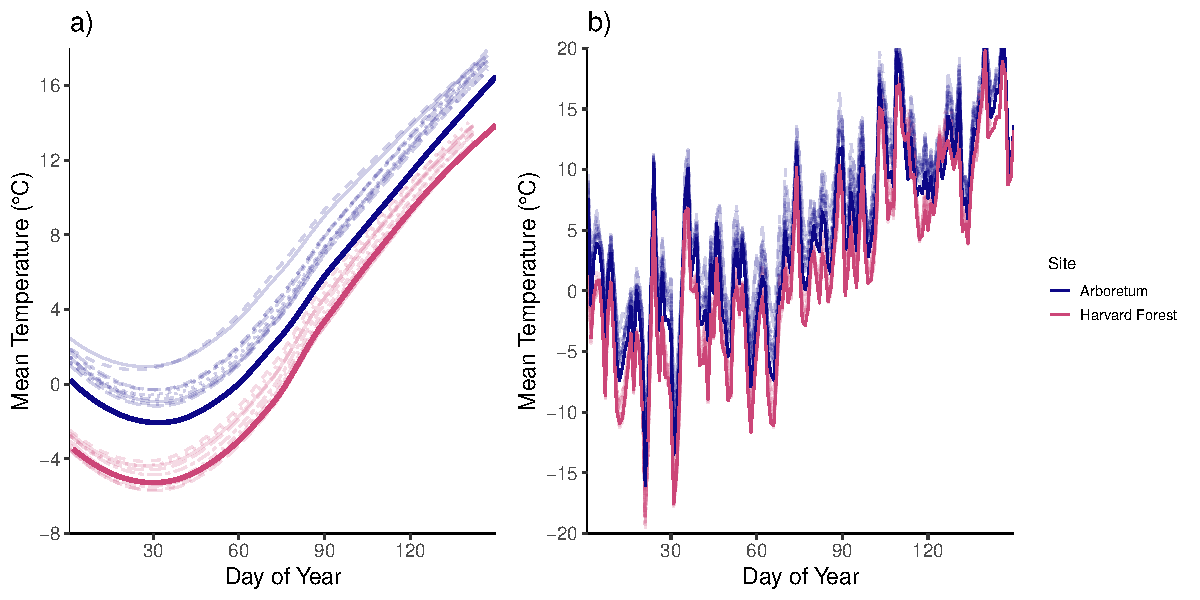
\includegraphics[width=16cm]{..//analyses/figures/climate_smooth&daily.pdf}
  \caption{Here we show a breakdown of the climate data across the two sites with darker lines representing weather station data and the lighter, more transparent lines of varying line types representing the hobo loggers: a) a series of smoothing splines of mean temperature with 90\% credible interval and b) actual mean temperature.}\label{fig:clim}
  \end{center}
  \end{figure}}
  
  
\begin{figure}[H]
      \centering
      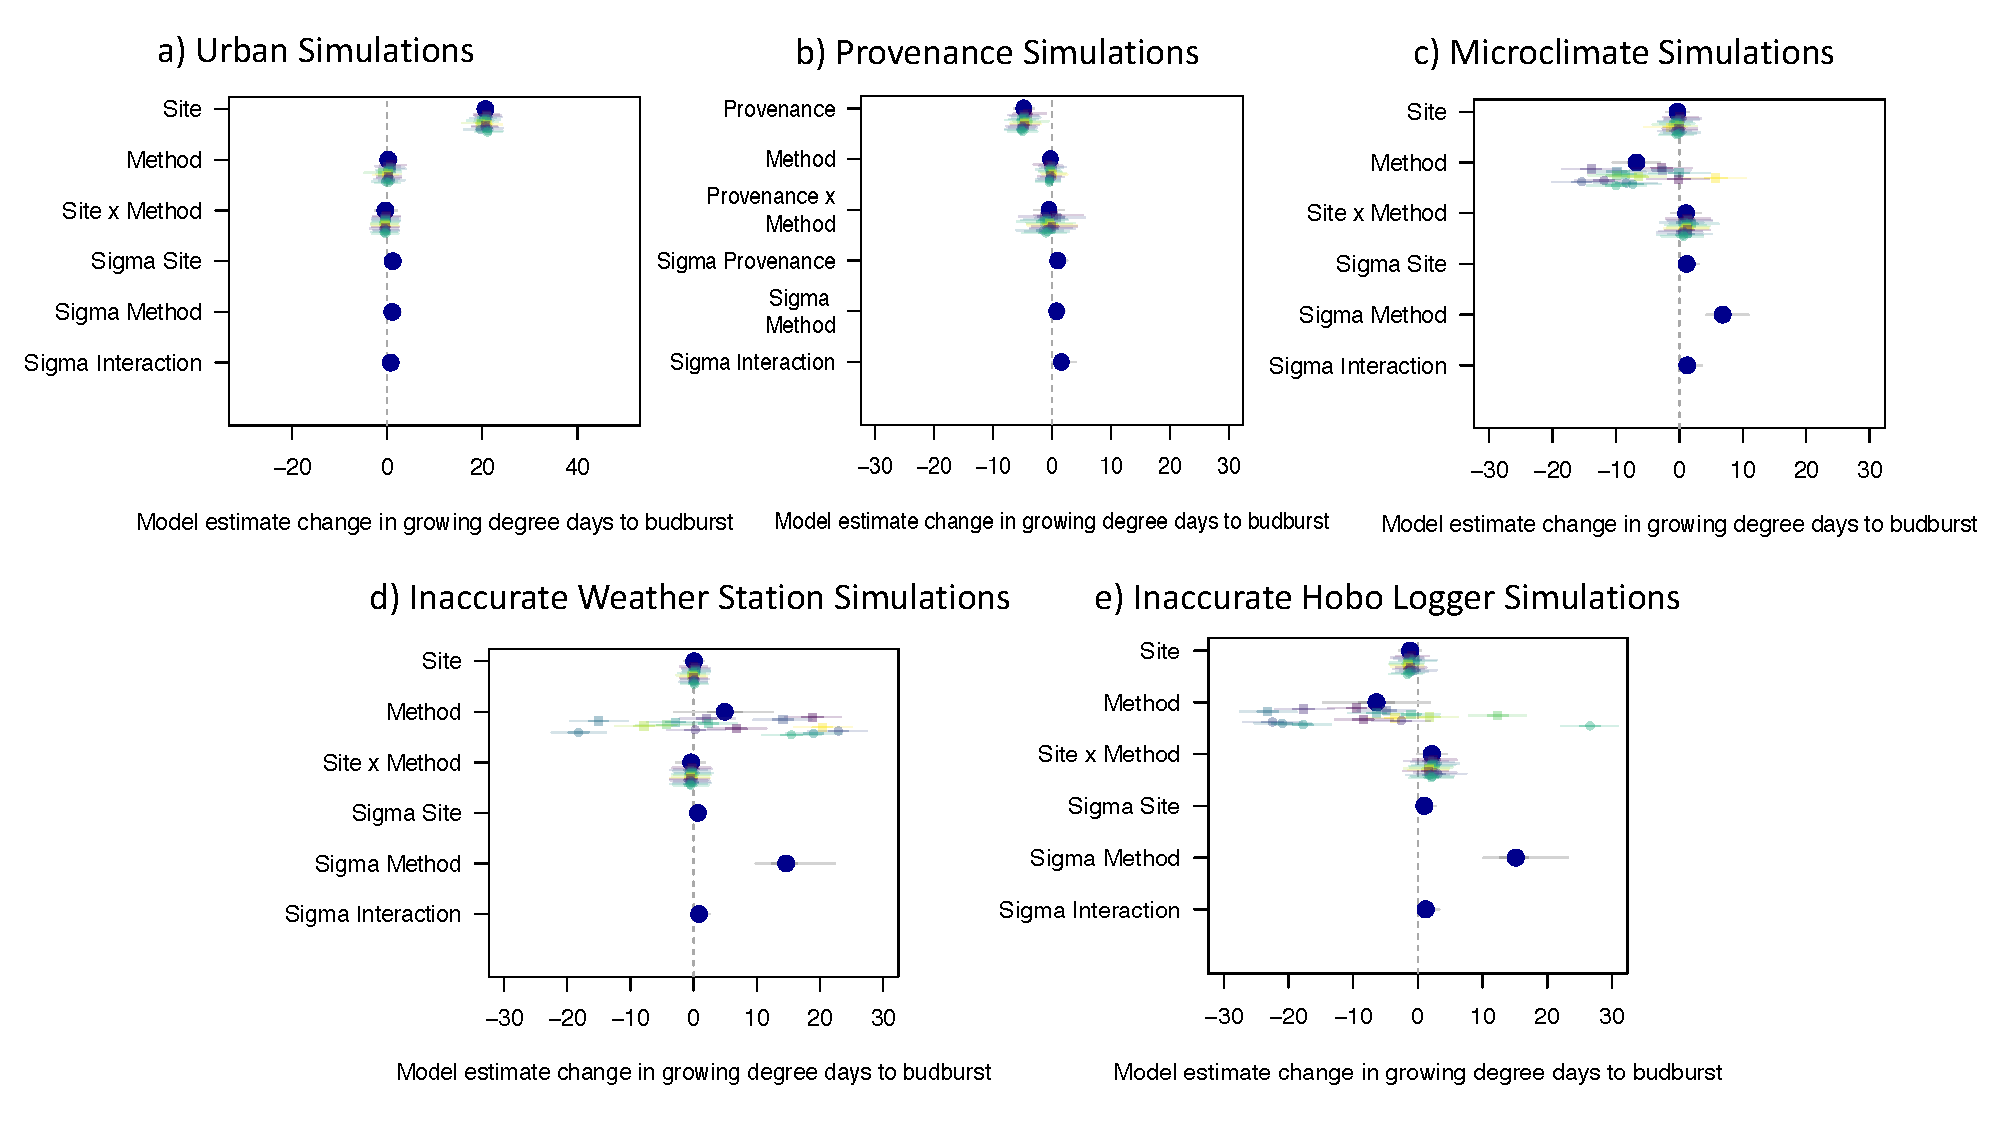
\includegraphics[width=16cm]{..//analyses/figures/muplot_sims.pdf}
\caption{ Simulations: using simulations we show (a) urban sites requiring more GDDs, (b) microclimate effects, (c) more northern provenance latitudes requiring fewer GDDs, (d) less accurate weather station data and (e) less accurate hobo logger data. We show the effects of site in (a), (b), (d) and (e) as a binary `urban' parameter with the urban site as `1' and the rural site as `0'. We also use a binary `weather station' parameter to represent the climate data method with weather station data reported as `1' and with hobo logger data as `0'. The intercept represents the hobo logger data for the rural forested site. More positive values indicate more GDDs are required for budburst whereas more negative values suggest fewer GDDs are required. Dots and thin lines show means and 90\% uncertainty intervals and thick lines show 50\% uncertainty intervals. See Tables \ref{tab:urban}, \ref{tab:micros}, \ref{tab:prov}, \ref{tab:noisyws} and \ref{tab:noisyhobo} for full model output. }
\label{fig:musims}
\end{figure}
  

\begin{figure}[H]
    \centering
    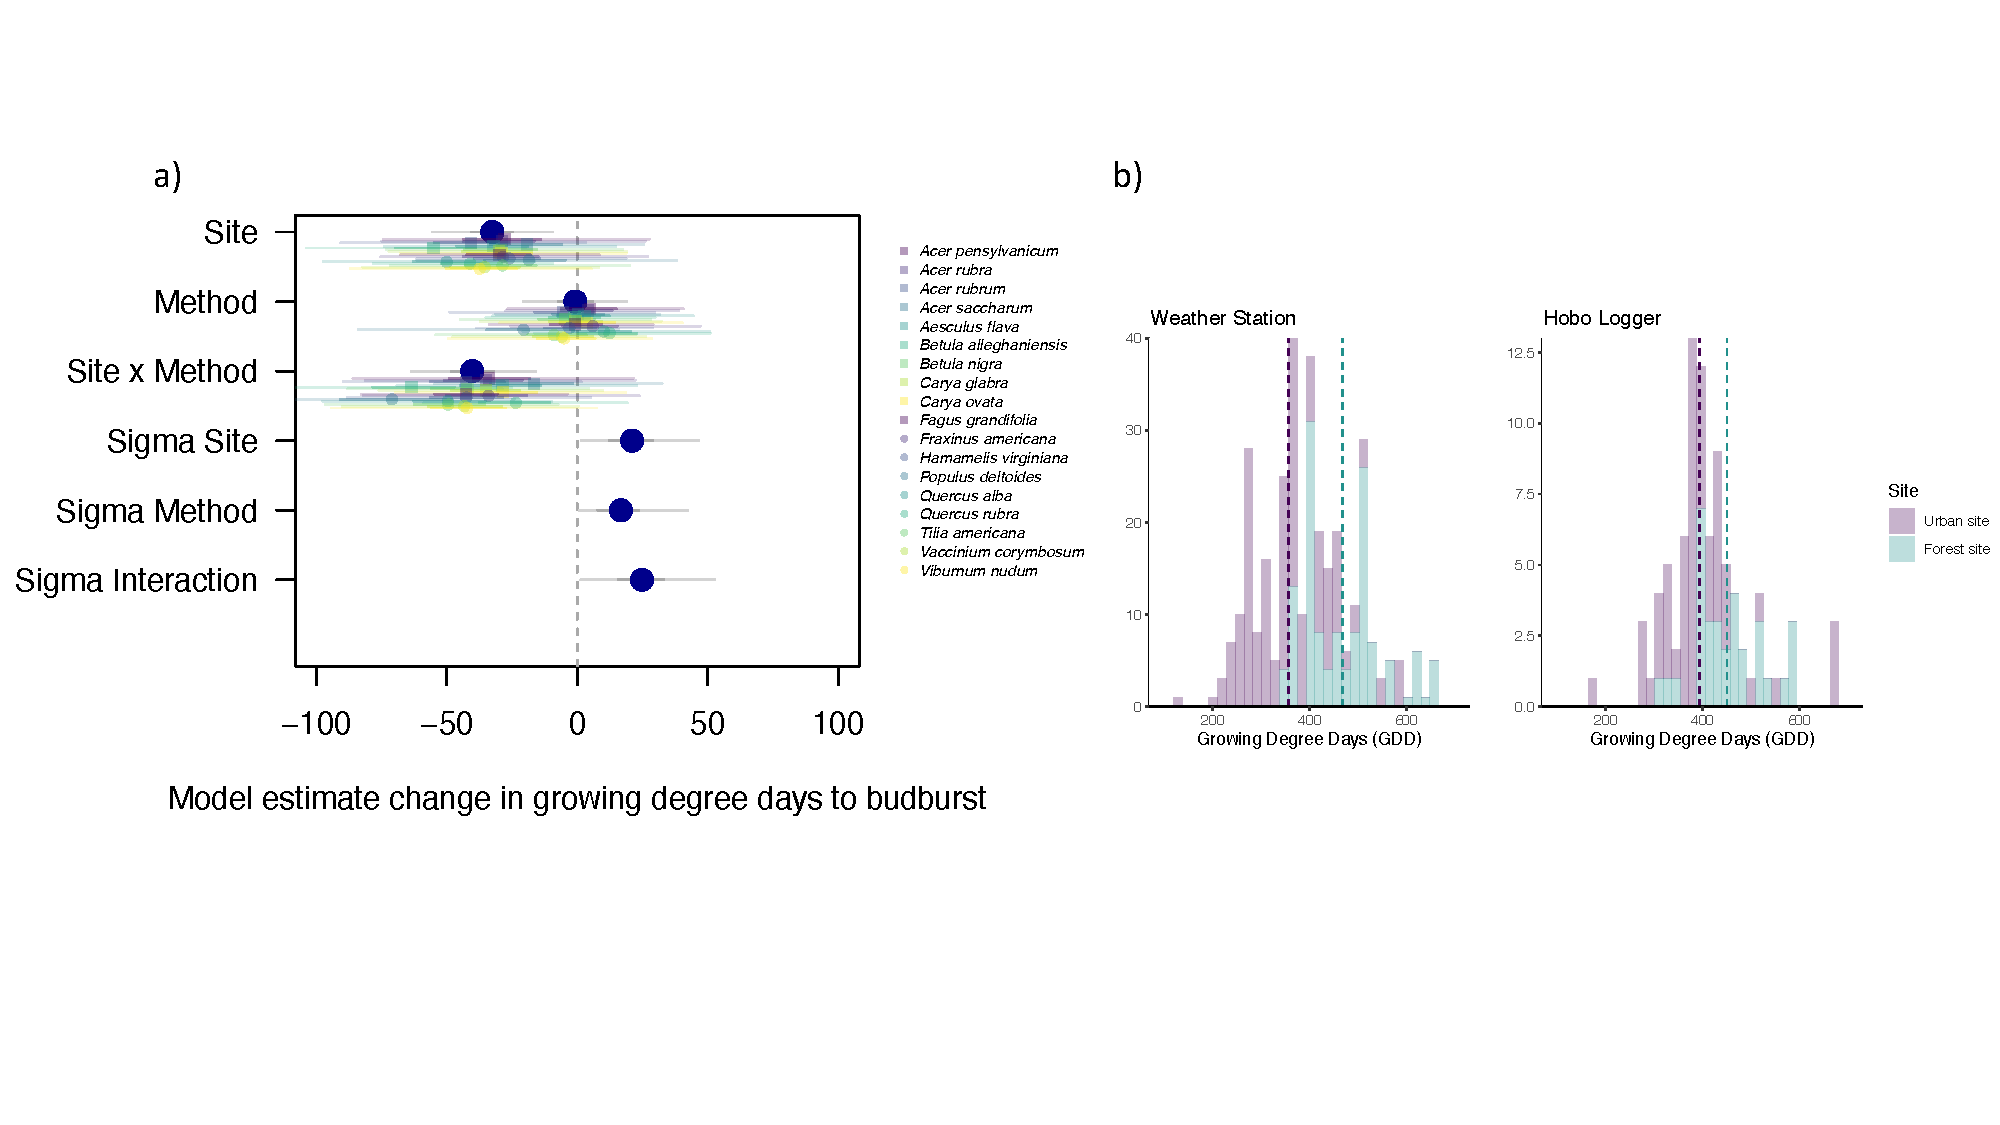
\includegraphics[width=16cm, trim=0cm 5cm 0cm 0cm,]{..//analyses/figures/muandgdd.pdf}
\caption{ Empirical Data: Using real data, we show (a) the effects of site (again using a binary predictor with the urban arboretum site reported as `1' and the rural forested site reported as `0') and climate data method (as a binary predictor with weather station data as `1' and hobo logger data as `0') on growing degree days (GDDs) until budburst. The intercept represents the hobo logger data for the rural forested site. More positive values indicate more GDDs are required for budburst whereas more negative values suggest fewer GDDs are required. Dots and thin lines show means and 90\% uncertainty intervals and thick lines show 50\% uncertainty intervals. See Table \ref{tab:real} for full model output. We also show (b) histograms of GDDs at the urban arboretum and rural forested site using weather station data and hobo logger data.}
\label{fig:real}
\end{figure}

\begin{figure}[H]
      \centering
      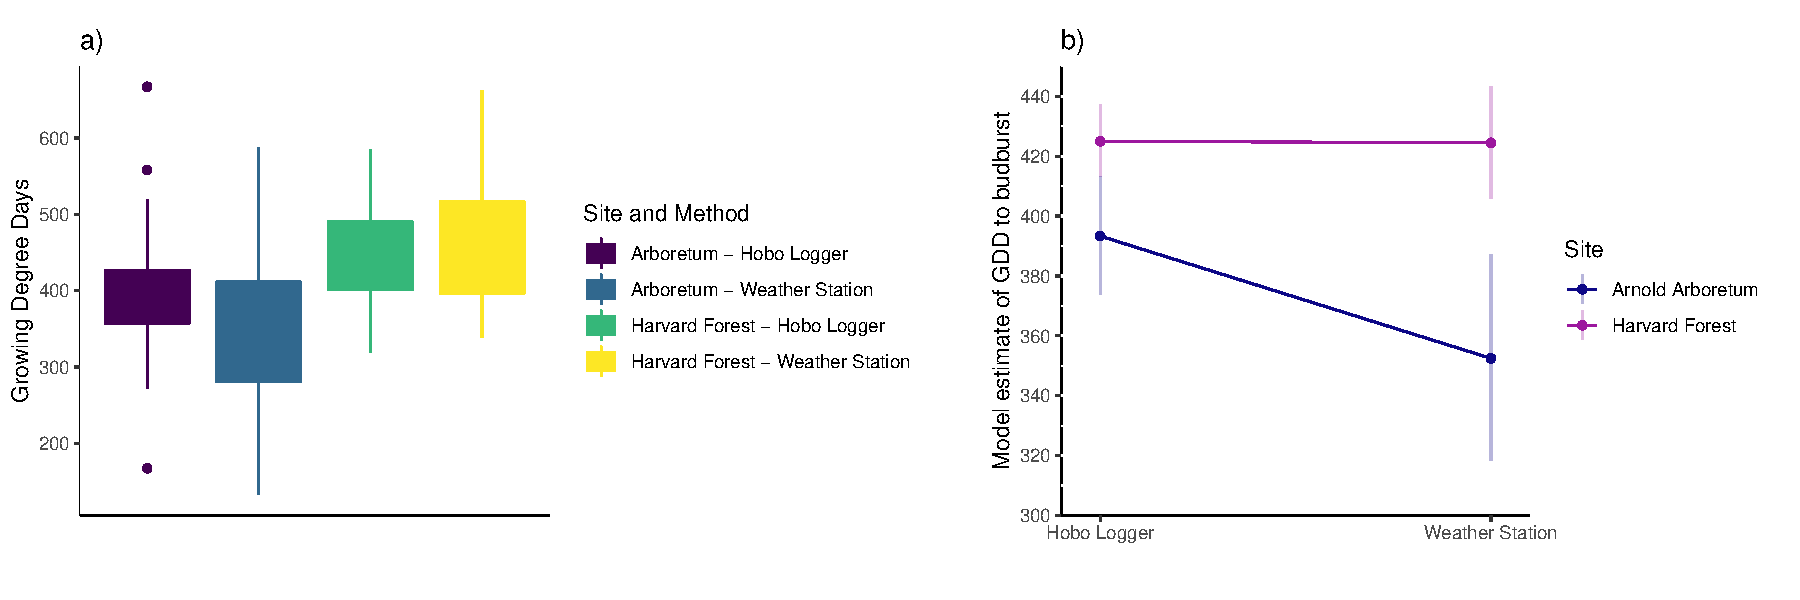
\includegraphics[width=16cm]{..//analyses/figures/gdd_interaction.pdf}
\caption{ We show effects of site (urban arboretum site versus forested rural site) by climate data method (weather station data versus hobo logger data) on growing degree days (GDDs) until budburst (a) as a boxplot across each method and site combination using raw data and (b) using model output to show the mean estimates for each site and method with 50\% uncertainty intervals shown as errorbars.}
\label{fig:interaction}
\end{figure}


\begin{figure}[H]
    \centering
    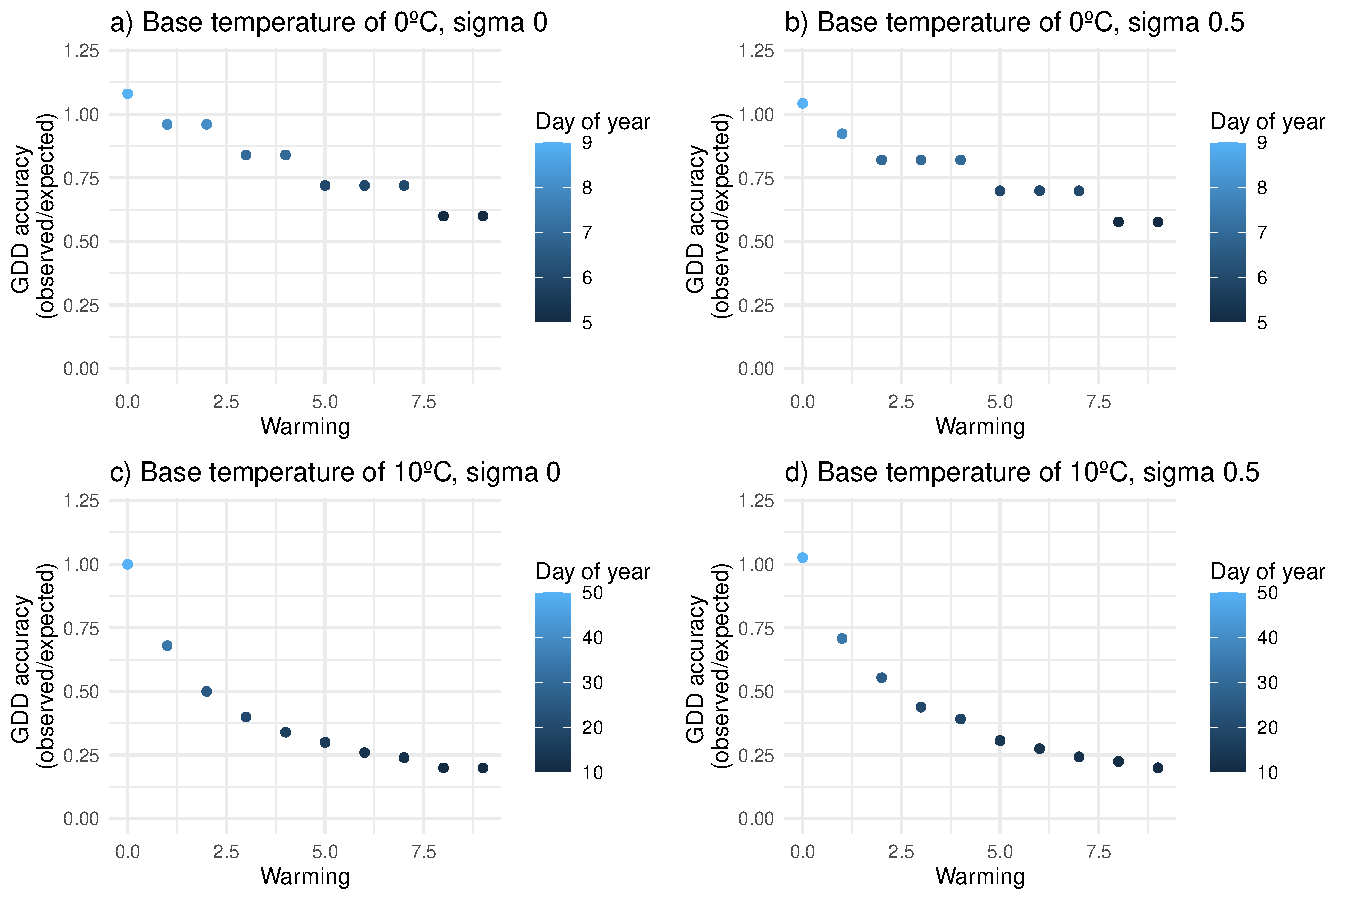
\includegraphics[height=8cm, width=12cm]{..//analyses/figures/gddratio_warming.pdf}
\caption{Using simulated data, we show how GDD measurement accuracy changes with warming (i.e., from 0$^{\circ}$C to 10$^{\circ}$C) using a base temperature of (a) 0$^{\circ}$C and a sigma of 0.1$^{\circ}$C, (b) 0$^{\circ}$C and a sigma of 0.5$^{\circ}$C, (c) 10$^{\circ}$C and a sigma of 0.1$^{\circ}$C and (d) 10$^{\circ}$C and a sigma of 0.5$^{\circ}$C. GDD accuracy is measured as the observed GDD divided by the expected GDD. }
\label{fig:warming}
\end{figure}

  
  

\end{document}
